\chapter{Introduction}
\label{chap:introduction}

\section{Logo detection and recognition}
\label{sec:logodet-intro}

Logo detection and recognition is a Computer Vision (CV) task that consists of two steps: localize logos in the image (i.e. to find the coordinates of the object relative to the image) and identify the detected logo (i.e. to produce in output the brand name associated with that logo).

The first studies in this field date back to 1993 \cite{doermann1993logo}, yet this task is becoming increasingly important in a variety of applications. Some examples of studies relative to this problem aimed to: monitor the brand visibility on social media \cite{7492197}; protect the intellectual property on e-commerce platforms, known as intellectual property protection (IPP) \cite{jin2020open}; develop online video advertising systems \cite{cheng2017video}; and help the development of autonomous checkout systems in retail environments \cite{mata2022standardsim}.

There are several challenges in logo detection and recognition, starting from the fact that a symbol composed by text and images can be considered a logo, but there is no formal definition of what a logo is. In fact, logos can be created from text using a lot of different typographic styles, any particular graphic consisting of many colors, or even a combination of the two.
There is a huge variety of logos and this problem has both high intra-class and inter-class variations, since the same brand can have very different logos (e.g. only a stylized text version and a graphic version) and logos which belong to different brands might look very similar.

Since many new brands are constantly being created and each brand has its own logo, it is necessary to develop systems that keep up with the creation of new logos. A method for logo detection and recognition should take into account this particular aspect of the problem and should properly recognize each new logo.

For this reason, there is the need to develop a system which is able to adapt to these changes where standard closed-set classification techniques would fail. One possible approach could be to train a new classifier each time a new logo is created. This method is very inefficient and unfeasible for large scale datasets of logos. Moreover, retraining a model in such a way would require to store examples, since both the data from the previous logos and the new ones would be needed.

Open set logo recognition allows models to
detect logos that are not available during the training stage. In this way, it is possible to overcome the problems discussed above. As a consequence, systems in which logo detection and recognition is performed in an open environment have been proposed in the literature \cite{fehervari2019scalable, li2022seetek}.

\section{Class incremental learning}
Incremental learning aims to develop artificially intelligent
systems that can continuously learn to address new tasks
from new data while preserving knowledge learned from
previously learned tasks \cite{masana2020class}. This way of learning is inspired from natural systems which are intrinsically incremental \cite{wu2019large}.

The main problem in incremental learning is known as the stability-plasticity dilemma and it holds for both artificial and biological neural systems. The idea is that a learning system requires plasticity for the integration of new knowledge, but also stability in order to prevent the forgetting of previous knowledge \cite{mermillod2013stability}. Excessive plasticity would lead to forget all the previous knowledge (referred to as catastrophic forgetting \cite{grossberg2013adaptive}), whereas too much stability would prevent the ability to learn novel concepts. The main point is to achieve a trade-off between stability and plasticity. 

Many real-world applications require incremental learning capabilities: intelligent robots during their lifetime \cite{thrun1995lifelong}, face recognition systems \cite{li2017incremental} and autonomous driving \cite{pierre2018incremental}. Logo detection and recognition is another example where class incremental learning (CIL) is well suited to address the problem, considering the constant creation of new logos discussed in the previous section. Using this technique it is possible to create a system which detects and recognizes an initial set of logos and, when necessary, enriches the acquired knowledge.

\section{Proposed approach}

\begin{figure}
    \begin{center}
        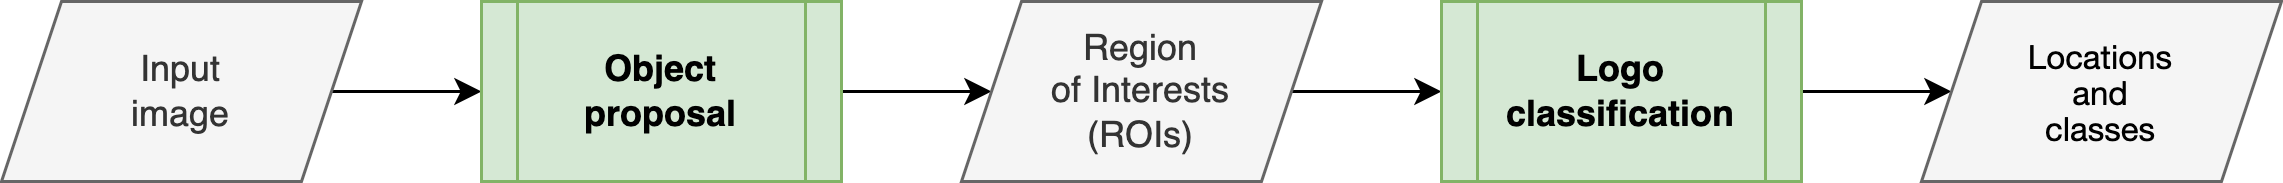
\includegraphics[width=\columnwidth]{images/pipeline.drawio.png}
    \end{center}
    \caption{Simplified system pipeline.}
    \label{fig:system-pipeline}
\end{figure}


The goal of this thesis is to develop a system that can detect and recognize 
a large number of different logos present in an image. An important factor that is considered in this work is the incremental learning aspect. This means that the system is trained on an initial set of logos and, when necessary, it is possible to enrich its knowledge to recognize new logos. This is done by taking advantage of state of the art incremental learning techniques.

The proposed system is conceptually simple, it consists of two deep learning models and follows a pipeline composed of two main steps, shown in \autoref{fig:system-pipeline}:

\begin{enumerate}
    \item \textbf{Object Proposal} for logo detection, performed by the class-agnostic logo detector
    \item \textbf{Classification} for logo recognition, performed by the CIL classifier
\end{enumerate}

In the first step, the model is a class-agnostic logo detector based on YOLOv5 \cite{glenn_jocher_2021_5563715}. In this context, class-agnostic means that the logo detector is only responsible for identifying a generic logo, while the actual classification is not done by the detector, but is delegated to the second model that produces the logo class as output.
Given an input image, the purpose of this first step is to produce as many cropped portions of it as there are logos in the image. These cropped regions are called region proposals and correspond to what the model considers to be logos.

The second step exploits the Regions of Interest (RoIs) generated by the detector and proceeds with the actual recognition of logos, this step is purely a classification task.
Here the problem is to recognize new logos which are created over time. To do so, the model is initially trained on all the logos that are available up to that time. Then, the knowledge of the model is updated to include a new set of logos. These updates of the knowledge are called incremental learning steps, and a crucial aspect of integrating new knowledge is the ability to do so in such way that the model does not forget its previous knowledge. As a consequence, the developed model uses incremental learning techniques that allow it to recognize new logos (classes).

Unlike the second step, we can say that there is no need to develop a detector with incremental learning techniques. This is justified by the fact that the idea of what a generic logo is can be learned and well-approximated using only an initial set of logos. The subsequent creation of new logos will not disrupt the general idea of a logo, therefore, there is no need to change the knowledge initially learned.

\vspace{1.5\baselineskip}
This thesis is structured as follows: starting from this introduction, the second chapter describes the state of the art regarding object detection, logo recognition and class incremental learning algorithms; the third chapter describes the dataset used to tackle this problem; the fourth chapter is a detailed description of the development and the techniques adopted; the fifth chapter describes the experiments and results obtained using the developed system; the last chapter is relative to the conclusions of this work and some considerations about future works.